\chapter{空间向量代数(Spatial Vector Algebra)}
\section{数学基础知识(Mathematical Preliminaries)}
\subsection{向量与向量空间 (Vectors and Vector Spaces)}

在空间向量代数中，线性代数将向量定义为向量空间中的元素。四种向量空间：

\begin{itemize}
    \item $\mathbb{R}^n$ --- \textbf{坐标向量 (Coordinate vectors)}：通常表示为 $n \times 1$ 的列矩阵，用于代表其他抽象向量。
    \item $E^n$ --- \textbf{欧几里得向量 (Euclidean vectors)}：定义了欧几里得内积，具有长度（Magnitude）和方向（Direction）的属性。
    \item $M^n$ --- \textbf{空间运动向量 (Spatial motion vectors)}：描述刚体运动属性，如速度和加速度。在三维动力学中通常使用 $M^6$。
    \item $F^n$ --- \textbf{空间力向量 (Spatial force vectors)}：描述力、冲量和动量。在三维动力学中通常使用 $F^6$。
\end{itemize}
这里面上标表示空间的维数。除了上述空间外，还会用到一类空间，即所谓的$m \times n$维向量空间，由$m \times n$矩阵构成。记作：$\mathbf{R}^{m \times n}$
\begin{tcolorbox}[colback=blue!6, title=上下标注意]
上标(Hats)的条件：\\当需要区分空间向量和三维向量时，给三维向量加帽子。比如\textbf{$\hat{\bm{v}}$}\\当需要区分坐标向量和抽象向量时，在坐标向量下面加下划线，比如$\underline{\bm{v}}$
\end{tcolorbox}

\subsection{对偶空间 (The Dual of a Vector Space)}

设 $V$ 为一个向量空间，其对偶空间记作 $V^*$。它们具有以下性质：
\begin{itemize}
    \item $V^*$ 与 $V$ 维度相同。
    \item $V$ 和 $V^*$ 之间定义了标量积（Scalar Product），记作 $\boldsymbol{u} \cdot \boldsymbol{v}$，其中 $\boldsymbol{u} \in V^*, \boldsymbol{v} \in V$。
    \item \textbf{物理关联}：$M^n$ 和 $F^n$ 互为对偶空间。如果 $\boldsymbol{m} \in M^6$ 是速度，$\boldsymbol{f} \in F^6$ 是力，则 $\boldsymbol{m} \cdot \boldsymbol{f}$ 的物理意义是该力产生的\textbf{功率}。
\end{itemize}

\subsection{对偶基与对偶坐标 (Dual Bases and Dual Coordinates)}

\subsubsection{互惠条件 (Reciprocity Condition)}
设 $\mathcal{D} = \{\boldsymbol{d}_1, \dots, \boldsymbol{d}_n\}$ 是 $U$ 的基，$\mathcal{E} = \{\boldsymbol{e}_1, \dots, \boldsymbol{e}_n\}$ 是 $V$ 的基。若它们满足以下条件，则称其为对偶基：
\begin{equation}
\boldsymbol{d}_i \cdot \boldsymbol{e}_j = \begin{cases} 1 & \text{if } i=j \\ 0 & \text{otherwise} \end{cases}
\end{equation}

\subsubsection{对偶坐标下的运算}
在对偶坐标系下，标量积可以表示为坐标向量的转置相乘：
\begin{equation}
\boldsymbol{u} \cdot \boldsymbol{v} = \underline{\boldsymbol{u}}^{\text{T}} \underline{\boldsymbol{v}}
\end{equation}
其中 $\underline{\boldsymbol{u}}$ 和 $\underline{\boldsymbol{v}}$ 分别是向量在对偶基下的坐标表示。

\subsubsection{坐标变换}
若 $\mathbf{X}$ 是作用于运动向量的变换矩阵，则作用于对偶空间（力向量）的对应变换矩阵 $\mathbf{X}^*$ 为：
\begin{equation}
\mathbf{X}^* = \mathbf{X}^{-\text{T}}
\end{equation}
\subsection{对偶空间性质的数学推导}

\subsubsection{标量积的数学定义}
设 $V$ 是 $n$ 维向量空间（对应 $M^n$），$V^*$ 是其对偶空间（对应 $F^n$）。定义标量积为一个映射 $\langle \cdot, \cdot \rangle: V^* \times V \to \mathbb{R}$。该映射必须满足以下数学性质：
\begin{enumerate}
    \item \textbf{双线性（Bilinearity）}：对于 $\forall a, b \in \mathbb{R}$，有 $\langle a\boldsymbol{u}_1 + b\boldsymbol{u}_2, \boldsymbol{v} \rangle = a\langle \boldsymbol{u}_1, \boldsymbol{v} \rangle + b\langle \boldsymbol{u}_2, \boldsymbol{v} \rangle$。
    \item \textbf{非退化性（Non-degeneracy）}：若对于所有 $\boldsymbol{u} \in V^*$ 都有 $\langle \boldsymbol{u}, \boldsymbol{v} \rangle = 0$，则必有 $\boldsymbol{v} = \mathbf{0}$。这保证了 $V$ 中的每一个运动分量在 $V^*$ 中都有唯一的对应力分量来产生响应。
\end{enumerate}

\subsubsection{对偶基的构造与互惠性推导}
设 $\mathcal{E} = \{\boldsymbol{e}_1, \dots, \boldsymbol{e}_n\}$ 是 $V$ 的一组基。由于标量积是非退化的，根据线性代数基本定理，在 $V^*$ 中必然存在唯一的一组基 $\mathcal{D} = \{\boldsymbol{d}_1, \dots, \boldsymbol{d}_n\}$，使得：
\begin{equation}
\langle \boldsymbol{d}_i, \boldsymbol{e}_j \rangle = \delta_{ij}
\end{equation}
其中 $\delta_{ij}$ 为 Kronecker delta 符号。
\textbf{证明}：任一向量 $\boldsymbol{v} \in V$ 可表示为 $\boldsymbol{v} = \sum v_j \boldsymbol{e}_j$。
则其第 $i$ 个分量可以通过与对偶基做标量积提取出来：
\begin{equation}
\langle \boldsymbol{d}_i, \boldsymbol{v} \rangle = \langle \boldsymbol{d}_i, \sum_j v_j \boldsymbol{e}_j \rangle = \sum_j v_j \langle \boldsymbol{d}_i, \boldsymbol{e}_j \rangle = v_i
\end{equation}
这证明了在对偶坐标系下，标量积在数值上等同于坐标向量的点积 $\underline{\boldsymbol{u}}^{\text{T}} \underline{\boldsymbol{v}}$。

\subsubsection{坐标变换阵 $\mathbf{X}^* = \mathbf{X}^{-\text{T}}$ 的推导}
考虑线性变换（基底更迭）。设从基底 $\mathcal{E}$ 到 $\mathcal{E}'$ 的变换矩阵为 $\mathbf{X}$，即 $\boldsymbol{v}' = \mathbf{X}\boldsymbol{v}$。
为了保持数学形式的协变性（Covariance），标量积必须是基底无关的标量：
\begin{equation}
\underline{\boldsymbol{u}}'^{\text{T}} \underline{\boldsymbol{v}}' = \underline{\boldsymbol{u}}^{\text{T}} \underline{\boldsymbol{v}}
\end{equation}
将 $\underline{\boldsymbol{v}}' = \mathbf{X}\underline{\boldsymbol{v}}$ 代入上式：
\begin{equation}
\underline{\boldsymbol{u}}'^{\text{T}} (\mathbf{X} \underline{\boldsymbol{v}}) = \underline{\boldsymbol{u}}^{\text{T}} \underline{\boldsymbol{v}}
\end{equation}
由于该式对所有 $\underline{\boldsymbol{v}}$ 均成立，移项合并得：
\begin{equation}
(\underline{\boldsymbol{u}}'^{\text{T}} \mathbf{X} - \underline{\boldsymbol{u}}^{\text{T}}) \underline{\boldsymbol{v}} = 0 \implies \underline{\boldsymbol{u}}'^{\text{T}} \mathbf{X} = \underline{\boldsymbol{u}}^{\text{T}}
\end{equation}
对等式两边取转置：
\begin{equation}
\mathbf{X}^{\text{T}} \underline{\boldsymbol{u}}' = \underline{\boldsymbol{u}} \implies \underline{\boldsymbol{u}}' = (\mathbf{X}^{\text{T}})^{-1} \underline{\boldsymbol{u}} = \mathbf{X}^{-\text{T}} \underline{\boldsymbol{u}}
\end{equation}
由此得出，对偶空间的变换矩阵必然是原空间变换阵的逆转置 $\mathbf{X}^* = \mathbf{X}^{-\text{T}}$。


\subsection{算子与并矢 (Operators and Dyadics)}

\subsubsection{算子 $\boldsymbol{a}\cdot$ 与 $\boldsymbol{a}\times$}
\begin{itemize}
    \item $\boldsymbol{a}\cdot$ 是一个算子，将向量 $\boldsymbol{b}$ 映射为标量 $\boldsymbol{a} \cdot \boldsymbol{b}$。
        \item $\boldsymbol{a}\times$ 是一个算子，将向量 $\boldsymbol{b}$ 映射为跨乘向量 $\boldsymbol{a} \times \boldsymbol{b}$。在坐标表示下，$\boldsymbol{a}\times$ 表现为一个方阵。即一个斜对称矩阵（或者叫反对称矩阵）。
        \begin{equation}
            \boldsymbol{a}_{\times} = \begin{bmatrix} 0 & -a_3 & a_2 \\ a_3 & 0 & -a_1 \\ -a_2 & a_1 & 0 \end{bmatrix}
        \end{equation}
\end{itemize}

\subsection{并矢与并矢张量 (Dyads and Dyadics)}
形式如 $\boldsymbol{a}\boldsymbol{b}\cdot$ 的表达式称为\textbf{并矢 (Dyad)}。它是一个线性算子，映射规则如下：
\begin{equation}
(\boldsymbol{a}\boldsymbol{b}\cdot) \boldsymbol{c} = \boldsymbol{a}(\boldsymbol{b} \cdot \boldsymbol{c})
\end{equation}
一个一般的线性映射 $\mathbf{L}$ 可以表示为 $r$ 个线性无关并矢的和，称为\textbf{并矢张量}：
\begin{equation}
\mathbf{L} = \sum_{i=1}^r \boldsymbol{a}_i \boldsymbol{b}_i \cdot
\end{equation}
在空间向量代数中，这种形式常用于表示\textbf{空间惯性张量}。

\subsection{算子与并矢的张量积表示}
一个并矢 $\boldsymbol{a}\boldsymbol{b}\cdot$ 在数学上对应于张量积 $\boldsymbol{a} \otimes \boldsymbol{b}$，其中 $\boldsymbol{a} \in U, \boldsymbol{b} \in V^*$。
其作用于向量 $\boldsymbol{c} \in V$ 的线性映射定义为：
\begin{equation}
(\boldsymbol{a} \otimes \boldsymbol{b})(\boldsymbol{c}) = \boldsymbol{a} \langle \boldsymbol{b}, \boldsymbol{c} \rangle
\end{equation}
空间惯性张量 $\mathbf{I}$ 便是这种形式的求和 $\sum \boldsymbol{a}_i \boldsymbol{b}_i \cdot$，它建立了从 $M^6$ 到 $F^6$ 的映射。

\section{空间速度 (Spatial Velocity)}
为了描述刚体 $B$ 的运动，我们选择空间中一个任意固定的原点 $O$ 。在此参考点下，刚体的运动由一对 3D 向量完整指定：
\begin{itemize}
    \item $\bm{\omega}$：\textbf{角速度向量}，描述刚体绕过 $O$ 点轴线的旋转 。
    \item $\bm{v}_O$：\textbf{线速度向量}，指代刚体上当前与 $O$ 点重合的点的瞬时速度 。
\end{itemize}
此时，刚体可被视为在以线速度 $\bm{v}_O$ 平移的同时，绕着穿过 $O$ 点的轴以角速度 $\bm{\omega}$ 旋转 。
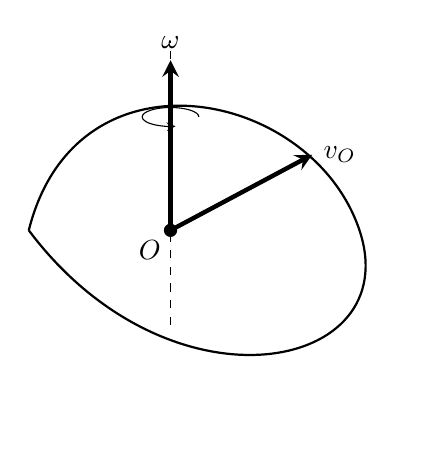
\begin{tikzpicture}[>=stealth, scale=1.2]
    % 1. 绘制刚体外形（简单的闭合曲线）
    \draw[thick] (-1.5,0) .. controls (-1,2) and (1.5,1.5) .. (2,0) 
                 .. controls (2.5,-1.5) and (0,-2) .. (-1.5,0);
    
    % 2. 定义基点 O
    \coordinate (O) at (0,0);
    \fill (O) circle (2pt);
    \node[below left] at (O) {$O$};

    % 3. 绘制线速度 v_O (橙色或深色)
    % 线速度是平移分量，通常画在 O 点上
    \draw[->, ultra thick] (O) -- (1.5, 0.8) node[right] {$\bm{v}_O$};

    % 4. 绘制旋转轴（虚线）
    \draw[dashed] (0,-1) -- (0,2);

    % 5. 绘制角速度 \omega (向上)
    \draw[->, ultra thick] (O) -- (0, 1.8) node[above] {$\bm{\omega}$};

    % 6. 简单的旋转小圆弧指示
    \draw[->] (0.3, 1.2) arc (0:280:0.3 and 0.1);
\end{tikzpicture}

\subsection{速度场公式 (Velocity Field)}
基于上述描述，刚体上任意一点 $P$ 的速度 $\bm{v}_P$ 可由以下公式计算：
\begin{equation}
\bm{v}_P = \bm{v}_O + \bm{\omega} \times \vec{OP} \tag{2.1}
\end{equation}
其中 $\vec{OP}$ 是点 $P$ 相对于点 $O$ 的位置向量 。该公式定义了一个向量场，即刚体 $B$ 的\textbf{速度场} 。虽然 $\bm{v}_O$ 取决于 $O$ 的选择，但整个速度场是刚体运动的固有属性 。\\
我说白了就是刚体上每个点都有自己的速度大小和方向，这些大小和方向构成一个向量场。\\
来吧，我们接下来将要开始狂飙了。\\
显然我们在一个笛卡尔坐标系中，可以这样表示那两个至关重要的速度：线速度和角速度。就像这样。\\$\bm{\omega}=\omega_x\bm{i}+\omega_y\bm{j}+\omega_z\bm{k}$\\
$\bm{v_O}=v_{Ox}\bm{i}+v_{Oy}\bm{j}+v_{Oz}\bm{k}$\\
这样我们把两个三维的速度整合为一个六维的速度。即下面的表示。

\subsubsection{Plücker 坐标表示}
引入以 $O$ 为原点的笛卡尔坐标系 $O_{xyz}$，定义标准正交基 $\{\bm{i}, \bm{j}, \bm{k}\}$ 。刚体的 6 自由度运动可以分解为六个基本运动：绕 $x, y, z$ 轴的旋转以及沿 $x, y, z$ 方向的平移 。

由此定义 \textbf{Plücker 基底} $\mathcal{D}_O \subset \mathsf{M}^6$：
\begin{equation}
\mathcal{D}_O = \{ \bm{d}_{Ox}, \bm{d}_{Oy}, \bm{d}_{Oz}, \bm{d}_x, \bm{d}_y, \bm{d}_z \} \tag{2.2}
\end{equation}
空间速度向量 $\hat{\bm{v}}$ 及其在 $\mathcal{D}_O$ 下的坐标向量为：
\begin{equation}
\hat{\bm{v}}_O = \begin{bmatrix} \omega_x \\ \omega_y \\ \omega_z \\ v_{Ox} \\ v_{Oy} \\ v_{Oz} \end{bmatrix} = \begin{bmatrix} \bm{\omega} \\ \bm{v}_O \end{bmatrix} \tag{2.4}
\end{equation}
这里 $\hat{\bm{v}}$ 是 $\mathsf{M}^6$ 空间中的一个元素，它将刚体的角速度和线速度统一在一个 6D 向量中 。


\begin{figure}[h]
    \centering
    % --- 图 (a) 开始 ---
    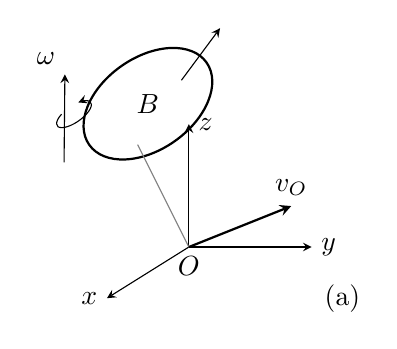
\begin{tikzpicture}[>=stealth, scale=1.3]
        % 坐标轴
        \draw[->] (0,0) -- (-0.8,-0.5) node[left] {$x$};
        \draw[->] (0,0) -- (1.2,0) node[right] {$y$};
        \draw[->] (0,0) -- (0,1.2) node[right] {$z$};
        \node[below] at (0,0) {$O$};

        % 刚体 B 及其旋转分量
        \begin{scope}[shift={(-0.4,1.4)}, rotate=35]
            \draw[thick] (0,0) ellipse (0.7 and 0.45);
            \node at (0,0) {$B$};
            % 角速度 omega
            \draw[->] (-1.0,0) -- (-0.5,0.7) node[above left] {$\bm{\omega}$};
            \draw[->] (-0.75,0.4) arc (120:420:0.2 and 0.08);
            % 刚体上的一个速度方向
            \draw[->] (0.4,0) -- (1.0,0.2);
        \end{scope}

        % 连接线
        \draw[thin, gray] (0,0) -- (-0.5,1.0);
        
        % 线速度 v_O
        \draw[->, thick] (0,0) -- (1.0,0.4) node[above] {$\bm{v}_O$};

        \node at (1.5, -0.5) {(a)};
    \end{tikzpicture}
    \hspace{1.5cm} % 两个图之间的间距
    % --- 图 (b) 开始 ---
    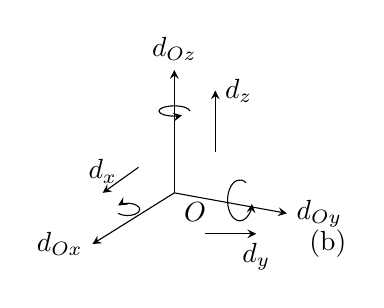
\begin{tikzpicture}[>=stealth, scale=1.3]
        \coordinate (O) at (0,0);
        \node[below right] at (O) {$O$};

        % Z 轴及位移
        \draw[->] (O) -- (0,1.2) node[above] {$\bm{d}_{Oz}$};
        \draw[->] (0.15,0.8) arc (0:300:0.15 and 0.05); 
        \draw[->] (0.4,0.4) -- (0.4,1.0) node[right] {$\bm{d}_{z}$};

        % X 轴及位移 (左下)
        \draw[->] (O) -- (-0.8,-0.5) node[left] {$\bm{d}_{Ox}$};
        \draw[->] (-0.35,0.25) -- (-0.7,0) node[above] {$\bm{d}_{x}$};
        \draw[->] (-0.55,-0.2) arc (220:500:0.12 and 0.06);

        % Y 轴及位移 (右下)
        \draw[->] (O) -- (1.1,-0.2) node[right] {$\bm{d}_{Oy}$};
        \draw[->] (0.3,-0.4) -- (0.8,-0.4) node[below] {$\bm{d}_{y}$};
        \draw[->] (0.7,0.1) arc (60:350:0.12 and 0.2);

        \node at (1.5, -0.5) {(b)};
    \end{tikzpicture}
    \caption{刚体运动学向量分解示意图}
\end{figure}




\subsection{应用举例与物理特性}

\subsubsection{Example 2.1: 向量场的线性叠加}
若 $\hat{\bm{v}}_1$ 和 $\hat{\bm{v}}_2$ 是两个空间速度，其对应的速度场分别为 $\bm{V}_1$ 和 $\bm{V}_2$ 。根据空间向量空间的线性性质，它们的合成速度 $\hat{\bm{v}}_{sum} = \hat{\bm{v}}_1 + \hat{\bm{v}}_2$ 对应的速度场满足线性叠加原理：
\begin{equation}
\bm{V}_{sum}(P) = \bm{V}_1(P) + \bm{V}_2(P) \quad (\forall P) \tag{2.5}
\end{equation}
这说明 $6\text{D}$ 空间向量的加法运算，完美映射了三维物理空间中刚体运动的复合关系。

\subsubsection{Example 2.2: 坐标变换的不变性 (Invariance)}
空间向量的核心物理价值在于其\textbf{坐标无关性}。即使我们改变参考原点，空间向量作为一个几何实体是不变的。
研究原点从 $O$ 换到 $P$ 时的表现。假设 $P$ 的坐标在 $O$ 系下为 $(r, 0, 0)$，根据速度变换公式 (2.1)，点 $P$ 的线速度分量 $\bm{v}_P$ 计算如下：
\begin{equation}
\begin{bmatrix} v_{Px} \\ v_{Py} \\ v_{Pz} \end{bmatrix} = \bm{v}_O + \bm{\omega} \times \begin{bmatrix} r \\ 0 \\ 0 \end{bmatrix} = \begin{bmatrix} v_{Ox} \\ v_{Oy} + \omega_z r \\ v_{Oz} - \omega_y r \end{bmatrix}
\end{equation}

虽然坐标分量 $(v_{Px}, v_{Py}, v_{Pz})$ 发生了变化，但由于 Plücker 基底向量 $\mathcal{D}_P$ 同时也发生了对应的几何位移，两者的变化相互抵消。因此，空间向量 $\hat{\bm{v}}$ 保持不变。这种不变性使得我们可以像处理普通的 3D 向量一样，对 6D 空间向量进行代数运算，而不必时刻担心参考点的漂移。

\subsubsection{深度补充：运动螺旋 (Screw Theory) 的解释}
为了更深入理解空间速度，我们可以引入\textbf{螺旋理论}。空间速度 $\hat{\bm{v}}$ 实际上定义了一个螺旋运动：
\begin{itemize}
    \item \textbf{螺旋轴 (Screw Axis)}：刚体上所有速度方向与角速度 $\bm{\omega}$ 平行的点构成的直线。
    \item \textbf{节距 (Pitch)}：定义为线性速度沿轴向分量与角速度大小的比值 $h = \frac{\bm{\omega} \cdot \bm{v}_O}{\|\bm{\omega}\|^2}$。
\end{itemize}
这种几何视角解释了为什么空间速度只需要 6 个参数就能描述极其复杂的刚体三维运动。


\subsection{注意事项}
在空间向量代数中，速度向量 $\hat{\bm{v}}$ 通常将角速度放在前三个分量，线速度放在后三个分量 。这种排列与空间力（Spatial Force）的排列（力矩在前，线性力在后）互为对偶，使得两者的内积 $\hat{\bm{f}} \cdot \hat{\bm{v}}$ 正好等于功率。



\section{空间力 (Spatial Force)}

在空间向量代数中，作用于刚体 $B$ 上的力也可以通过一对 3D 向量来完整描述。给定一个任意选择的固定点 $O$，作用在刚体上的总力系可以等效为：
\begin{itemize}
    \item $\bm{f}$：\textbf{线性力 (Linear Force)}，其作用线通过点 $O$ 。
    \item $\bm{n}_O$：\textbf{力偶矩 (Couple)}，代表作用于刚体上的总力矩 。
\end{itemize}

\subsection{力矩变换公式}
若已知相对于点 $O$ 的力矩，则相对于空间中任意点 $P$ 的总力矩 $\bm{n}_P$ 为：
\begin{equation}
\bm{n}_P = \bm{n}_O + \bm{f} \times \vec{OP} \tag{2.6}
\end{equation}


\paragraph{对称性观察} 
你会发现公式 (2.6) 与速度变换公式 (2.1) 具有完全一致的数学结构。在此类比中：
\begin{itemize}
    \item 线性力 $\bm{f}$ 对应角速度 $\bm{\omega}$ 。
    \item 力偶矩 $\bm{n}_O$ 对应线速度 $\bm{v}_O$ 。
\end{itemize}
这种对称性是空间向量代数能够将动力学方程简化的核心原因。


\subsection{Plücker 坐标表示}
为了在 6D 空间中表达力，我们引入 Cartesian 坐标系 $O_{xyz}$，并将 $\bm{f}$ 与 $\bm{n}_O$ 分解为分量形式 ：
\begin{align*}
    \bm{n}_O &= n_{Ox}\bm{i} + n_{Oy}\bm{j} + n_{Oz}\bm{k} \\
    \bm{f} &= f_x\bm{i} + f_y\bm{j} + f_z\bm{k}
\end{align*}

定义 \textbf{Plücker 力基底} $\mathcal{E}_O = \{ \bm{e}_x, \bm{e}_y, \bm{e}_z, \bm{e}_{Ox}, \bm{e}_{Oy}, \bm{e}_{Oz} \} \subset \mathsf{F}^6$ 。其中：
\begin{itemize}
    \item 前三个基向量 ($\bm{e}_x, \bm{e}_y, \bm{e}_z$) 是沿坐标轴的单位力偶 。
    \item 后三个基向量 ($\bm{e}_{Ox}, \bm{e}_{Oy}, \bm{e}_{Oz}$) 是通过原点 $O$ 且沿坐标轴的单位线性力 。
\end{itemize}

空间力向量 $\hat{\bm{f}} \in \mathsf{F}^6$ 在该基底下的坐标向量表示为：
\begin{equation}
\hat{\bm{f}}_O = \begin{bmatrix} n_{Ox} \\ n_{Oy} \\ n_{Oz} \\ f_x \\ f_y \\ f_z \end{bmatrix} = \begin{bmatrix} \bm{n}_O \\ \bm{f} \end{bmatrix} \tag{2.9}
\end{equation}


\subsection{重要特性：不变性 (Invariance)}
虽然分量 $n_{Ox}, n_{Oy}, \dots$ 的具体数值取决于坐标系 $O_{xyz}$ 的位置和朝向，但由这些分量与基底向量组合而成的空间力向量 $\hat{\bm{f}}$ 作为一个整体是**不变的 (Invariant)** 。它代表了施加在刚体上的物理相互作用本身，不随观测者的参考系选择而改变 。

\subsection{总结：运动向量与力向量的对偶排列}
在笔记中需要特别注意分量的排列顺序：
\begin{table}[h]
\centering
\begin{tabular}{|c|c|c|}
\hline
\textbf{向量类型} & \textbf{前三个分量} & \textbf{后三个分量} \\ \hline
空间速度 $\hat{\bm{v}}$ & 角速度 $\bm{\omega}$ & 线速度 $\bm{v}_O$ \\ \hline
空间力 $\hat{\bm{f}}$ & 力偶矩 $\bm{n}_O$ & 线性力 $\bm{f}$ \\ \hline
\end{tabular}
\end{table}
这种“交叉对应”的排列方式保证了标量积（内积）具有明确的物理意义：
\begin{equation*}
    P = \hat{\bm{f}} \cdot \hat{\bm{v}} = \bm{n}_O \cdot \bm{\omega} + \bm{f} \cdot \bm{v}_O
\end{equation*}
即空间力和空间速度的乘积等于该力对刚体所做的**瞬时功率** 。

\section*{Plücker 表示法 (Plücker Notation)}

Plücker 坐标是 6D 向量的首选坐标系。该表示法将 Plücker 坐标与特定于速度（$\bm{v}$ 和 $\bm{\omega}$）及力（线性力和力矩向量）的符号相结合。

在一般情况下，若 $\hat{\bm{m}}$ 和 $\hat{\bm{f}}$ 分别表示 $\mathsf{M}^6$ 和 $\mathsf{F}^6$ 中的通用元素，则它们的 Plücker 坐标为：
\begin{equation}
\hat{\bm{m}}_O = \begin{bmatrix} m_x \\ m_y \\ m_z \\ m_{Ox} \\ m_{Oy} \\ m_{Oz} \end{bmatrix} = \begin{bmatrix} \bm{m} \\ \bm{m}_O \end{bmatrix} \quad \text{以及} \quad \hat{\bm{f}}_O = \begin{bmatrix} f_{Ox} \\ f_{Oy} \\ f_{Oz} \\ f_x \\ f_y \\ f_z \end{bmatrix} = \begin{bmatrix} \bm{f}_O \\ \bm{f} \end{bmatrix}
\end{equation}

我们应始终按照 \textbf{角量在前，线性量在后 (angular-before-linear)} 的顺序排列 Plücker 坐标；即三个角坐标始终排在最前面。

\section*{线向量与自由向量 (Line Vectors and Free Vectors)}

\begin{itemize}
    \item \textbf{线向量 (Line vector)}：由一条有向直线和一个幅值特征化（例如：纯转动、线性力）。它可以用五个数字来指定。
    \item \textbf{自由向量 (Free vector)}：由一个幅值和一个方向特征化（例如：纯平移、纯力偶）。它可以用三个数字来指定。
\end{itemize}

令 $\hat{\bm{s}}$ 为任一空间向量，$\bm{s}$ 和 $\bm{s}_O$ 为提供其 Plücker 坐标的两个 3D 坐标向量。基本事实如下：
\begin{itemize}
    \item 如果 $\bm{s} = \bm{0}$，则 $\hat{\bm{s}}$ 是一个自由向量。
    \item 如果 $\bm{s} \cdot \bm{s}_O = 0$，则 $\hat{\bm{s}}$ 是一个线向量。直线的方向由 $\bm{s}$ 给出，直线本身是满足 $\vec{OP} \times \bm{s} = \bm{s}_O$ 的点 $P$ 的集合。
    \item 任何空间向量（自由向量除外）都可以唯一地表示为一个线向量与一个平行自由向量之和。对于运动向量，其表达式为：
    \begin{equation}
    \begin{bmatrix} \bm{s} \\ \bm{s}_O \end{bmatrix} = \begin{bmatrix} \bm{s} \\ \bm{s}_O - h\bm{s} \end{bmatrix} + \begin{bmatrix} \bm{0} \\ h\bm{s} \end{bmatrix} \quad \text{其中} \quad h = \frac{\bm{s} \cdot \bm{s}_O}{\bm{s} \cdot \bm{s}}
    \end{equation}
\end{itemize}

在螺线理论（Screw Theory）中，最通用的刚体运动称为 \textbf{twist (旋量)}，最通用的力称为 \textbf{wrench (力旋量)}。自由向量幅值与线向量幅值的比值称为 \textbf{pitch (节距)}。

\subsubsection*{幅值 (Magnitude)}

空间向量在欧几里得意义上没有幅值。然而，对于四类空间向量可以定义有意义的幅值：转动、平移、线性力和力偶。幅值仅在每一类内部具有可比性。Plücker 基向量取决于所选的单位制。

\section{标量积 (Scalar Product)}

空间向量上的标量积定义要求一个参数必须是运动向量 ($\hat{\bm{m}} \in \mathsf{M}^6$)，另一个必须是力向量 ($\hat{\bm{f}} \in \mathsf{F}^6$)。
\begin{itemize}
    \item 表达式 $\hat{\bm{m}} \cdot \hat{\bm{m}}$ 和 $\hat{\bm{f}} \cdot \hat{\bm{f}}$ 是 \textbf{未定义 (not defined)} 的。
    \item 标量积在 $\mathsf{M}^6$ 和 $\mathsf{F}^6$ 之间建立了一种正式的 \textbf{对偶 (duality)} 关系：每个空间都是另一个空间的对偶空间。
\end{itemize}

$\mathsf{M}^6$ 和 $\mathsf{F}^6$ 上的对偶坐标系由两个基底 $\{\bm{d}_1, \dots, \bm{d}_6\} \subset \mathsf{M}^6$ 和 $\{\bm{e}_1, \dots, \bm{e}_6\} \subset \mathsf{F}^6$ 构成，满足：
\begin{equation}
\bm{d}_i \cdot \bm{e}_j = \begin{cases} 1 & \text{如果 } i = j \\ 0 & \text{否则} \end{cases}
\end{equation}

如果 $\underline{\bm{m}}$ 和 $\underline{\bm{f}}$ 在对偶坐标系中表示 $\hat{\bm{m}} \in \mathsf{M}^6$ 和 $\hat{\bm{f}} \in \mathsf{F}^6$，则：
\begin{equation}
\hat{\bm{m}} \cdot \hat{\bm{f}} = \underline{\bm{m}}^T \underline{\bm{f}}
\end{equation}

若矩阵 $\bm{X}$ 对运动向量执行坐标变换，而 $\bm{X}^*$ 对力向量执行相同的变换，则两者关系为：
\begin{equation}
\bm{X}^* = \bm{X}^{-T}
\end{equation}